% Created 2019-02-14 Thu 15:32
% Intended LaTeX compiler: pdflatex
\documentclass[11pt]{article}
\usepackage[utf8]{inputenc}
\usepackage[T1]{fontenc}
\usepackage{graphicx}
\usepackage{grffile}
\usepackage{longtable}
\usepackage{wrapfig}
\usepackage{rotating}
\usepackage[normalem]{ulem}
\usepackage{amsmath}
\usepackage{textcomp}
\usepackage{amssymb}
\usepackage{capt-of}
\usepackage{hyperref}
\usepackage{hyperref}
\hypersetup{colorlinks=true, allcolors=blue}
\author{Hassan Shabbir}
\date{\today}
\title{Editing Text With Vim}
\hypersetup{
 pdfauthor={Hassan Shabbir},
 pdftitle={Editing Text With Vim},
 pdfkeywords={},
 pdfsubject={},
 pdfcreator={Emacs 26.1 (Org mode 9.1.14)}, 
 pdflang={English}}
\begin{document}

\maketitle
\tableofcontents

\newpage

\section{The main text editors}
\label{sec:org2de6360}
There are two main (extensible) text editors for Unix and GNU/Linux\footnote{I'd just like to interject for a moment. What you usually refer
to as Linux, is in fact, GNU/Linux, or as I've recently taken to calling
it, GNU plus Linux. Linux is not an operating system unto itself, but 
rather another free component of a fully functioning GNU system made 
useful by the GNU corelibs, shell utilities and vital system components
comprising a full OS as defined by POSIX. (See GNU Linux copypasta.)}
operating systems. These are the VI and Emacs lines of text editors.

Both of these text editors are highly configurable and therefore are highly
recommended by many programmers, so much so that since their inception many
programmers have been in a "war", arguing over which text editor is
better.\footnote{See \href{https://en.wikipedia.org/wiki/Editor\_war}{The Editor Wars}.}
\subsection{VI}
\label{sec:org3ff856d}
VI (pronounced "vee-eye"), and other text editors based off of it are great at
creating and editing text. It is (usually) a basic text editor, however, newer
versions of it allow a user to customize it and get IDE-like features within
it.\footnote{This is usually not encouraged, especially at the beginning,
since having plugins hinder your ability to understand Vim, and are nice
to have and not necessarily mandatory for the functioning of Vim.} The main feature of VI is the way in which it allows a user to edit
text.
\subsection{GNU Emacs}
\label{sec:orgf3c4bda}
GNU\footnote{GNU stands for "GNU's Not Unix", a recursive acronym.} Emacs (pronounced "g'noo ee-maks") is a text editor that is extremely
configurable and allows for a lot more IDE-like features. This is due to the
fact that Emacs is a text editor written and extensible in the general purpose
functional programming language Lisp. Emacs can also emulate VI keybindings
using EVIL mode (EVIL stands for Extensible VI Layer). It is also interesting to
note that Richard Stallman,\footnote{\href{https://en.wikipedia.org/wiki/Richard\_Stallman}{Richard Stallman}.} the creator of GNU Emacs, also created the
first alternative to Unix, which was GNU, the Free Software Foundation, as well
as the GNU General Public Licence.

From here on out we will be talking about the VI line of editors. The curious
reader is encouraged to read more about Emacs, if interested.
\section{Which Vim version should I use?}
\label{sec:org73bdde6}
NOTE: There is almost no difference between these different text editors (for
our purposes) except for the information written below.

NOTE: I will assume that Vim/NeoVim is used for the rest of this file, but will
refer to it as Vim, since I am lazy.

There are three different VI versions you should be familiar with.
\subsection{VI}
\label{sec:orgb85423c}
VI\footnote{VI pronounced "vee-eye", also pronounced "vy" but that is an
unofficial pronunciation.} is the oldest text editor of the three\footnote{Technically, the "ed" and "ex" editors are even older, but are 
quite cumbersome to use. For example, they require you to print a range
of lines to be able to see them.}, which was created in
1976.\footnote{This is where the command mode in VI comes from, see below. 
Also, see \href{https://sanctum.geek.nz/arabesque/actually-using-ed/}{Actually Using Ed} for some extreme masochism.} VI is short for Visual, differentiating it from line editors. If
you plan to work with many servers, you should expect literally expect every
server to have it. It is very minimalistic so it won't tell you when you are in
insert mode in any way (see below), for example. This makes it harder to
understand for beginners, and doesn't have all the features of Vim.
\subsection{Vim}
\label{sec:org2c26de1}
Vim\footnote{Vim pronounced "vim".} is the newer version of VI, first released in 1991. Due to it being
very popular for a long time, and still is (last stable release: 17 May 2018),
it has many resources available on the internet for it. It is also recently
modern, so it shouldn't be too difficult to use. Therefore, whenever searching
for general vim resources use vim in the search terms.
\subsection{NeoVim}
\label{sec:org042c5c1}
NeoVim\footnote{NeoVim pronounced "neo-vim".} is the newest version of vim, first released in 2015. This has the
most interactive features and therefore is the one that I would recommend to new
users. For example, when you switch between different modes, the cursor changes,
helping you to remember which mode you are in.

\noindent\rule{\textwidth}{0.5pt}

\newpage

\section{Installing Vim/NeoVim}
\label{sec:orgfaa9b55}
Packages (programs) can easily be installed in any Linux distribution using the
command line. For example, to manage packages on Ubuntu Linux, use the package
manager \texttt{apt}. The full command to install Vim would then be \texttt{sudo apt install
vim}, and the command to install NeoVim would be \texttt{sudo apt install nvim}.\footnote{The command to both run and install it is \texttt{nvim} NOT \texttt{neovim}.}
\section{Modal editing with Vim}
\label{sec:org4b7b1a1}
The first thing you need to know about Vim is that there are four main modes in
which you operate. Each of these modes changes what the keys on your keyboard
will do.

In general, when editing text you will mostly be making small changes, and very
rarely do you create whole documents without mistakes from start to finish (\texttt{cat
> foo.txt} anyone?). For this reason, Vim is optimized for modifying text.
Understanding modal editing (along with composability, repeatability, and text
objects) is the key to understanding Vim.\footnote{For more on how vim works see this awesome answer on StackOverflow
\href{https://stackoverflow.com/questions/1218390/what-is-your-most-productive-shortcut-with-vim}{Your problem with Vim is that you don't grok vi}.}
\subsection{Normal Mode (Movement; Modification)}
\label{sec:org83212da}
Normal mode allows you to issue commands to Vim, which will then do something,
other than putting the key that you pressed into the file. When you first open a
file you will be in Normal Mode. Pressing keys such as \texttt{j} or \texttt{l} will move the
cursor rather than adding those letters to the file. You should almost always be
in Normal Mode since editing text requires the ability to move around the
document, and deleting, replacing, copying text, etc. which are all possible in
Normal mode. Thus this mode is called "normal" since it is the default mode when
using Vim. To get back into Normal Mode either use the escape key, or the key
combination control and the left square bracket keys.
\subsection{Insert Mode (Add Text)}
\label{sec:org7ad0192}
When opening a document with Vim, you will be in Normal Mode. To get into Insert
Mode, for example, you can press keys such as \texttt{i} or \texttt{a} and then you will be in
Insert Mode. If you are using NeoVim, you will see the cursor become thin, and
in both Vim and NeoVim, you will see \texttt{-{}-INSERT-{}-} at the bottom of the
terminal.\footnote{In VI you will neither see the cursor change nor the 
\texttt{-{}-INSERT-{}-} at the bottom.} You can then use the arrow keys to get to the location and press
the keys to add them to the document. To get back to Normal Mode press escape.
(This is not recommended but can help you get used to Vim. Movement commands
should be done using Normal Mode, not the arrow keys, allowing your hand to stay
on home row) You will notice that the cursor will become a block again in
NeoVim.
\subsection{Command Mode (System Commands; Ed commands)}
\label{sec:orgbb989cf}
For now, the most important command mode you need to know will be the commands
to exit Vim (which is accessible from Command Mode). This is such a problem for
Vim beginners that \href{https://stackoverflow.com/questions/11828270/how-to-exit-the-vim-editor}{this StackOverflow answer} has 4,000 upvotes, and over 1
Million views. First enter Normal mode by pressing the escape key, then press
\texttt{:}. You will now see a colon on the last line of the terminal. If you wish to
save your changes type \texttt{wq}, and then press enter. This command stands for write
(save) the file then quit Vim. If you wish to throw away your changes type \texttt{q!}
instead and then press enter.
\subsection{Visual Mode (Select Text)}
\label{sec:org8b6bc22}
Visual Mode is used for performing an operation over all of the characters in
the text. This can be useful when you don't know how to run operations using
text objects. Text objects allow you to refer to regions of text, such as "in
braces", "in tag", "all paragraph", etc. Text objects will replace most simple
uses of Visual Mode.

\begin{figure}[htbp]
\centering
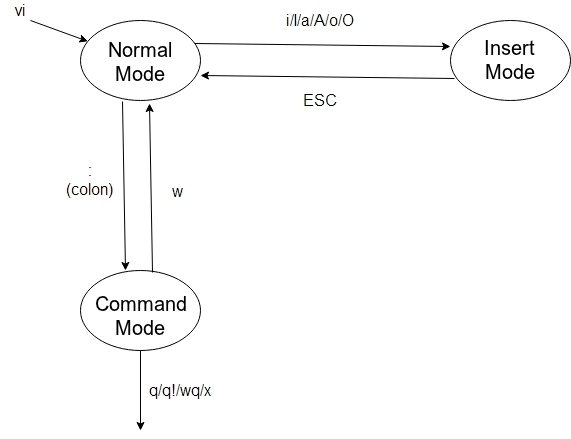
\includegraphics[width=.9\linewidth]{./modes.jpg}
\caption{\label{fig:org6630125}
General overview of Vim Modes. Will be covered in depth later.}
\end{figure}
\section{Vim editing commands}
\label{sec:org984a9f3}
NOTE: The 'Beginner' subheading will let you know which parts to focus on as a
beginner. Only learn the Beginner commands that you want. Then when you get
annoyed by inefficiency you can come back to learn more.

NOTE: Pressing the Escape key will return you back to Normal Mode from any mode.

NOTE: Vim uses mnemonic devices (ie. \texttt{d} stands for delete) to help you remember
what each command does. Use this to remember what each command does. Also,
commands that are related, but do something different are capitalized (\texttt{D}
deletes to the end of the line), and the default action is defined by the
repeated letter (such as \texttt{dd}\footnote{When you see characters, one after another, the keys should also 
be pressed one after another.} for delete with the default action, delete
line).

Sections will be in the form: CommandName (from StartingMode)

Commands will be in the form:
\begin{itemize}
\item \texttt{COMMAND}: (mnemonic device) Description of command
\end{itemize}
\subsection{Entering NeoVim (from bash prompt)}
\label{sec:org273ff0a}
You can enter NeoVim from the command line (not to be confused with Vim's
Command Mode) by typing \texttt{nvim file.txt}, replacing \texttt{file.txt} for the file you
want to edit. If the file doesn't exist, it will be created. You will now be in
NeoVim.

If you wish to use Vim, replace \texttt{nvim} in the command above with \texttt{vim}.
\subsection{Movement Commands (from Normal Mode)}
\label{sec:org74723c1}
\subsubsection{Character Movement}
\label{sec:org3f4c814}
\begin{enumerate}
\item Beginner
\label{sec:org375d376}
\begin{itemize}
\item \texttt{h}: Move cursor left
\item \texttt{j}: Move cursor down
\item \texttt{k}: Move cursor up
\item \texttt{l}: Move cursor right
\end{itemize}

The way to remember this is that the \texttt{h} key is on the left of the four keys,
\texttt{l} is on the right, \texttt{j} is written with the hook below the line, and \texttt{k} has
the vertical line above the line.

Character movement can also be prefixed with a number such as \texttt{5l}, to go 5
characters right.

\begin{figure}[htbp]
\centering
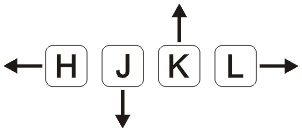
\includegraphics[width=.9\linewidth]{./hjkl.png}
\caption{\label{fig:org71e7755}
A graphical depiction of h, j, k, l}
\end{figure}
\end{enumerate}
\subsubsection{Line Movement}
\label{sec:orge769456}
\begin{enumerate}
\item Beginner
\label{sec:org849cda7}
\begin{itemize}
\item \texttt{\textasciicircum{}}: (This is from Regexes\footnote{Regexes, or regular expressions, are a way of doing things like 
parsing and substituting in a file. The regex \texttt{\textasciicircum{}hi} says to match the 
line starting with \texttt{hi} and the regex \texttt{\textasciicircum{}\$} says match the empty line 
(ie. the line that starts and ends with nothing in between).}) Go to start of line
\item \texttt{\$}: (This is from Regexes) Go to end of line
\end{itemize}
\end{enumerate}
\subsubsection{File Movement}
\label{sec:orgfdd2918}
\begin{enumerate}
\item Beginner
\label{sec:orgb0e1197}
\begin{itemize}
\item \texttt{gg}: (Go) Go to start of file
\item \texttt{G}: (Go) Go to end of file
\end{itemize}
\item Intermediate
\label{sec:orgc45db58}
\begin{itemize}
\item \texttt{50gg}: (Go) Go to line 50
\end{itemize}
\end{enumerate}
\subsubsection{Word Movement}
\label{sec:orgc8b7853}
\begin{enumerate}
\item Intermediate
\label{sec:org2f9538d}
Frankly, I used to just spam \texttt{h} and \texttt{l} for quite a while, so these commands
aren't strictly necessary.

\begin{itemize}
\item \texttt{w}: (Word) Go forward by one word
\item \texttt{b}: (Back) Go back by one word
\item \texttt{e}: (End) Go to the next end-of-word
\end{itemize}
\end{enumerate}
\subsubsection{Find Char Movement}
\label{sec:org8f2097e}
\begin{enumerate}
\item Beginner
\label{sec:orgd26e6a2}
\begin{itemize}
\item \texttt{fx}: (Find Char) Find character 'x' forwards
\item \texttt{;}: Run \texttt{f} / \texttt{F} again
\end{itemize}
\item Intermediate
\label{sec:orgd683064}
\begin{itemize}
\item \texttt{Fx}: (Find Char) Find character 'x' backwards
\item \texttt{,}: Run \texttt{f} / \texttt{F} again in opposite direction
\item \texttt{tx}: ('Til/Until) Go up until character 'x', forwards
\item \texttt{Tx}: ('Til/Until) Go up until character 'x', backwards
\end{itemize}
\end{enumerate}
\subsubsection{Search Term Movement}
\label{sec:org7f822fd}
\begin{enumerate}
\item Beginner
\label{sec:orgb7c9a70}
\begin{itemize}
\item \texttt{/}: Input search term, then press enter
\item \texttt{n}: (Next) Go to next location matching search term
\end{itemize}
\item Intermediate
\label{sec:org7328ab6}
\begin{itemize}
\item \texttt{N}: (Previous/Backwards Next) Go to previous location matching search term
\end{itemize}
\end{enumerate}
\subsection{Insert Commands (from Normal Mode)}
\label{sec:org8249e84}
These commands will change you automatically from Normal Mode to Insert Mode.
\subsubsection{Beginner}
\label{sec:org62fe27e}
\begin{itemize}
\item \texttt{i}: (Insert) Enter Insert Mode before current character
\item \texttt{I}: (Insert) Enter Insert Mode at the beginning of the line
\item \texttt{a}: (Append) Enter Insert Mode after current character
\item \texttt{A}: (Append) Enter Insert Mode at the end of the line
\end{itemize}
\subsubsection{Intermediate}
\label{sec:org1d2afa9}
\begin{itemize}
\item \texttt{o}: (Open) Enter Insert Mode at the end of the line
\item \texttt{O}: (Open) Enter Insert Mode at the end of the line
\end{itemize}
\subsection{Deletion Commands (from Normal Mode)}
\label{sec:org30367c3}
NOTE: The composable nature of Vim should be apparent in this section.
\subsubsection{Beginner}
\label{sec:org14422f5}
\begin{itemize}
\item \texttt{x}: Delete character under cursor
\item \texttt{dd}: (Delete, Default) Delete current line
\item \texttt{dw}: (Delete Word) Delete until the end of the word
\item \texttt{dfc}: (Delete Find 'c') Delete including the first 'c' on the right of the cursor
\item \texttt{diw}: (Delete In Word) Delete the whole word
\item \texttt{diW}: (Delete In Word) Delete the whole space delimited word
\end{itemize}
\subsubsection{Intermediate}
\label{sec:orge4bb342}
I can't really be bothered to count how many words I want to delete. I prefer
doing things like \texttt{dw..} instead, see below.
\begin{itemize}
\item \texttt{d3w}: (Delete Word) Delete 3 number of words, etc.
\end{itemize}
\subsection{Deletion Commands (from Visual Mode)}
\label{sec:org393f2e9}
\subsubsection{Beginner}
\label{sec:org5bdcad2}
\begin{itemize}
\item \texttt{d}: (Delete) Delete current visual selection
\item \texttt{x}: (Delete) Delete current visual selection
\end{itemize}
\subsection{Change Commands (from Normal Mode)}
\label{sec:orgefefc1b}
Change deletes something then puts you in Insert Mode to add text.
\subsubsection{Beginner}
\label{sec:org23c0b29}
\begin{itemize}
\item \texttt{cc}: (Change, Default) Delete line, then go into Insert Mode
\item \texttt{cw}: (Change Word) Delete until the end of the word, then go into Insert Mode
\item \texttt{ciw}: (Change In Word) Delete the whole word, then go into Insert Mode
\item \texttt{ciW}: (Change In Word) Delete the whole space delimited word, then go into Insert Mode
\end{itemize}
\subsubsection{Intermediate}
\label{sec:org3d8c56c}
I can't really be bothered to count how many words I want to change. I prefer
doing things like \texttt{cw..} instead, see below.
\begin{itemize}
\item \texttt{c3w}: (Change Word) Delete 3 number of words, etc., then go into Insert Mode
\end{itemize}
\subsection{Yank (Copy) Commands (from Normal Mode)}
\label{sec:orgd47c32e}
NOTE: To copy text to use in other applications, use the \texttt{"+} prefix, which may
not work in VI/Vim, also see registers below.
\subsubsection{Beginner}
\label{sec:orgcd181fe}
\begin{itemize}
\item \texttt{yy}: (Yank, Default) Yank (copy) the current line, for Vim use only
\item \texttt{yiw}: (Yank) Yank (copy) the current line, for Vim use only
\item \texttt{"+yy}: (Yank, Default) Yank (copy) the current line, for any application
\item \texttt{"+yiw}: (Yank) Yank (copy) the current line, for any application
\end{itemize}
\subsection{Yank (Copy) Commands (from Visual Mode)}
\label{sec:org72c993d}
\subsubsection{Beginner}
\label{sec:orga744b65}
\begin{itemize}
\item \texttt{y}: (Yank) Yank (copy) current visual selection
\end{itemize}
\subsection{Paste Commands (from Normal Mode)}
\label{sec:orgdc2c1da}
\subsubsection{Beginner}
\label{sec:orgec1d14e}
\begin{itemize}
\item \texttt{p}: (Paste) Paste the last deletion/yank
\end{itemize}
\subsection{Paste Commands (from Visual Mode)}
\label{sec:orga159a32}
\subsubsection{Beginner}
\label{sec:org8990b60}
\begin{itemize}
\item \texttt{p}: (Paste) Paste, replacing current visual selection
\end{itemize}
\subsection{Undo Command (from Normal Mode)}
\label{sec:org5c282ec}
\subsubsection{Beginner}
\label{sec:orgf1dbc35}
\begin{itemize}
\item \texttt{u}: (Undo) undo last change
\end{itemize}
\subsection{Visual Mode Commands (from Normal Mode)}
\label{sec:org2325ecb}
First, enter Visual Mode using any of the below, then make the selection using
the movement commands as you would from Normal Mode. Then run the command on the
selection, such as yank, delete, etc.
\subsubsection{Beginner}
\label{sec:org84eb261}
\begin{itemize}
\item \texttt{v}: (Visual) Enter character-wise Visual Mode
\item \texttt{V}: (Visual) Enter line-wise Visual Mode
\end{itemize}
\subsubsection{Intermediate}
\label{sec:org1b10b0f}
\begin{itemize}
\item \texttt{ctrl-v}: (Visual) Enter block-wise Visual Mode
\end{itemize}

NOTE: To comment out lines, use block-wise selection with \texttt{ctrl-v}, then press
\texttt{I}, and type the character comment (\texttt{//} for example), and hit escape. It can
also be used as a poor man's version of a macro (see below). Another way would
be to use the Vim Commentary plugin (see below), with the command \texttt{gc}.
\subsection{Command Mode (from Normal Mode)}
\label{sec:orga5b5806}
\subsubsection{Beginner}
\label{sec:org9985536}
All of the below can be simplified to just \texttt{:w} and \texttt{:q}, since Vim will warn
you if you try to quit with unsaved changes.

\begin{itemize}
\item \texttt{:w}: (Write) Write the file
\item \texttt{:q}: (Quit) Quit Vim, without having modified the file
\item \texttt{:q!}: (Quit!) Quit Vim, throwing away modifications
\item \texttt{:wq}: (Write-Quit) Write the file, then quit Vim
\item \texttt{:x}: (Exit) Shorthand for \texttt{:wq}
\end{itemize}
\subsubsection{Intermediate}
\label{sec:org94120d9}
\begin{itemize}
\item \texttt{:! date}: (\texttt{!} is similar to \texttt{|}) Run bash command \texttt{date} and show the result without adding to file
\item \texttt{:r! date}: (Read) Run bash command \texttt{date} and read in the result into the file
\item \texttt{:s/foo/bar/g}\footnote{The text \texttt{foo} can be either a literal string or a regex, 
such as \texttt{\textasciicircum{}foo}.}: (Substitute) Substitute 'foo' with 'bar', globally (ie. each occurrence)
\end{itemize}
\subsection{Command Mode (from Visual Mode)}
\label{sec:org0306858}
Visually select text then enter Command Mode using \texttt{:}. NOTE: you will see
\texttt{:'<,'>}\footnote{So the command will run in the range \texttt{x,y}, and a \texttt{'a} refers to
the mark a, with the \texttt{<} referring to the first and \texttt{>} referring to the
last selection. So all together it says "run the command from the 
beginning of the selection to the end of the selection."} instead. This just tells Vim to run the command over the whole
selection.
\subsubsection{Intermediate}
\label{sec:orgb90fd1d}
\begin{itemize}
\item \texttt{:'<,'>! wc -l}: Run bash command \texttt{wc -l} on visually selected text, replacing with the result
\end{itemize}
\section{Composability and repeatability}
\label{sec:org4ec45e3}
This section should introduce you to even more advanced concepts.
\subsection{Text Objects}
\label{sec:org8104490}
NOTE: All text objects can be used with delete, yank, copy, etc. "In" deletes
the text inside, while "All" deletes quotes, braces, and a single space (so the
spaces around it end up balanced).
\subsubsection{Beginner}
\label{sec:org53a5ffd}
\begin{itemize}
\item \texttt{iw}: (In Word)
\item \texttt{aw}: (All Word)
\item \texttt{is}: (In Sentence)
\item \texttt{as}: (All Sentence)
\item \texttt{ip}: (In Paragraph)
\item \texttt{ap}: (All Paragraph)
\item \texttt{i"}: (In Quote)
\item \texttt{a"}: (All Quote)
\item \texttt{i\}}: (In Brace)
\item \texttt{a\}}: (All Brace)
\item \texttt{it}: (In Tag) Used in HTML
\item \texttt{at}: (All Tag) Used in HTML
\end{itemize}
\subsection{Dot (\texttt{.}) command}
\label{sec:org5f2d554}
\subsubsection{Beginner}
\label{sec:orgdd59bc1}
The dot command repeats the last complete command that you ran. For example if
you changed a word to "Hi" using \texttt{ciwHi} and then escape, you can change another
word to "Hi" using the dot command.

Expanding on the above, one way\footnote{The other way would be to run a search and replace, such as 
\texttt{:s/foo/bar/g}, which would replace all occurrences of \texttt{foo} with \texttt{bar}.} to quickly rename variables would be to
first search for a variable using \texttt{/}, then using \texttt{ciw} to change the variable
to something else. Finally, repeat this change all throughout the document using
\texttt{n} to go to the next instance, and \texttt{.} to apply the change.
\subsection{Number Prefixes}
\label{sec:org2711568}
\subsubsection{Intermediate}
\label{sec:org85eed6e}
Most commands can be prefixed, meaning you can run commands like \texttt{d5w} which
will delete the next 5 words.
\subsection{Macros}
\label{sec:orgd783c59}
\subsubsection{Intermediate}
\label{sec:orgec3b026}
Macros can be used for creating groups of repeatable commands. In other words,
start the macro, run general commands (ie. \texttt{w} rather than \texttt{llllllll}), stop the
macro, run the macro previously defined on the text you want. The steps are:

\begin{enumerate}
\item \texttt{qa}: Record Macro in register \texttt{a}, see below
\item \texttt{q}: While recording, it will end the macro
\item \texttt{@a}: Run Macro in register \texttt{a}
\end{enumerate}

Fun fact: you can also define recursive\footnote{Here's a quick introduction to recursion. Recursion is defining 
something in terms of what you are defining. For example, a directory 
can contain multiple files and multiple directories. A math example 
would be an equation like \texttt{x = 1 + x}, and replacing x on the right with
\texttt{1 + x} giving us \texttt{x = 1 + 1 + x}, and continuing to infinity would give
us \texttt{x = 1 + 1 + 1 + 1 + ...}. A similar expansion can be carried out 
on the acronym \texttt{GNU}, left as an exercise for the reader.} macros, (works in NeoVim). This
allows you to create a single macro that runs forever (of course, Vim will stop
the macro at the end of the document, for example). An example of this is the
following key sequences: \texttt{qaV\textasciitilde{}j@aq@a}\footnote{Usually the \texttt{q} register is used for macros, but this can get
confusing when first starting out. The command would then be \texttt{qqV\textasciitilde{}j@qq@q}.}, which switches the case of every
character until the end of the document.
\subsection{Registers}
\label{sec:orgf9d83dd}
\subsubsection{Intermediate}
\label{sec:org024f897}
The most important part about registers is that the \texttt{"+}\footnote{The \texttt{"} is used to retrieve registers, with \texttt{+} referring to 
the name of the register to be accessed, (in this case it is the 
special "global register").} prefix is used
to store the global clipboard, which can be accessed by any program. Frankly, I
don't use any register other than the global one.

Other actions, such as yanks and deletions can be prefixed with a register, for
later retrieval.

A useful combination is using registers for editing a macro you wrote. To
continue from the macros section, you can write an incorrect macro, paste it
into the file, modify it, copy it back to the register, and then run that macro.
This seems quite difficult, but there can be really long macros that you would
rather go through the above to change a character than to remake the macro from
the beginning.
\section{{\bfseries\sffamily TODO} Extending Vim for yourself}
\label{sec:orga9909d0}
\subsection{Configuration File}
\label{sec:org28aa64f}
To change the default behaviour of Vim, and to keep it even after quitting, you
must modify a configuration (also known as a dot file\footnote{Because the file starts with a \texttt{.}, I know, so original.}) file for Vim. For
GNU/Linux and NeoVim users this file is \texttt{\textasciitilde{}/.config/nvim/init.vim}, for Vim users
the file is \texttt{\textasciitilde{}/.vimrc}. If you use Windows, the file will be \texttt{\_vimrc}\footnote{\href{https://superuser.com/questions/86246/where-should-the-vimrc-file-be-located-on-windows-7}{Locate Home in Windows}.} (in
the home directory in Windows).

For example, typing \texttt{:colorscheme elflord}\footnote{To find a colour scheme you like from the preinstalled colour 
schemes, go to \href{https://stackoverflow.com/questions/7331940/how-to-get-the-list-of-all-installed-color-schemes-in-vim}{List installed colorschemes}.} from Normal Mode, will change
the colour scheme to elflord for the current Vim session. Once you close Vim
this setting will be gone. To save this setting, save the following lines in the
configuration file as:

\begin{verbatim}
" Set colour scheme to elflord 
colorscheme elflord 
\end{verbatim}

Notice the lack of a colon at the beginning of the line. The \texttt{"} indicates a
line comment.

Here are some other settings you may wish to add to your Vim configuration
file.\footnote{This is mostly taken from \href{https://github.com/amix/vimrc}{Amix's Vimrc}.} In general, you should always copy the comments along with the
actual code. (NOTE: always understand what every command does before adding it
to your configuration file.)

The below file is also available as \texttt{configuration.vim} at
\href{https://github.com/Hassan-Shabbir/vim-introduction}{Hassan-Shabbir/vim-introduction}.

\begin{verbatim}
" Enable filetype plugins, such as syntax highlighting for files. 
filetype plugin indent on

" Actually enable syntax highlighting. 
syntax enable

" Set autoread to true. When a file is changed from the outside, 
" the file will be reloaded. 
set autoread

" With a map leader it's possible to do extra key combinations 
" like '<leader>w' saves the current file. 'mapleader' is 
" usually the backslash key ('\'), however, below we set it 
" to the ',' key, since it is easier to reach.
let mapleader = ","

" This is how you would define "in normal mode, if I press 
" the leader key (see above), followed by the 'w' key, 
" map it to be the same as writing the file".
nmap <leader>w :w!<cr>

" Set a space of 3 lines between the cursor and the top/bottom 
" of the window, making it easier to get the context of the code. 
set so=3

" Turn on a completion menu on the bottom. Used when you try to 
" tab-complete something in command mode. 
set wildmenu set wildmode=list:longest,full

" Configure backspace so it acts as it should act. Namely, 
" allow backspace to delete new lines, delete past the start 
" of insert mode, and delete autoindent.
set backspace=eol,start,indent

" Ignore case when searching, so '/hi' will match 'hi' in the 
" text, along with 'Hi'. 
set ignorecase

" If a case is used, however, search match using case. So 
" '/Hi' will only match 'Hi', and not 'hi', (since we 
" explicitly told the case). 
set smartcase

" Highlight search results. 
set hlsearch

" Make search act like search in modern browsers. 
set incsearch

" Don't redraw while executing macros (for performance). 
set lazyredraw

" Return to last edit position when opening files 
" NOTE: Put this all on one line 
au BufReadPost * 
  if line("'\"") > 1 && line("'\"") <= line("$") 
  | exe "normal! g'\"" | endif
\end{verbatim}

\subsection{Plugins}
\label{sec:org68acf4e}
These are a few plugins that I would consider quite useful.

\begin{itemize}
\item \href{https://github.com/junegunn/vim-plug}{Vim Plug}: Vim plugin manager
\end{itemize}
To be able to use the below plugins you need to install a plugin manager, this
is the one I personally use, (no real reason).

\begin{itemize}
\item \href{https://github.com/tpope/vim-sensible}{Vim Sensible}: set default settings for Vim
\end{itemize}
This is useful for starting off in Vim. (Not needed for NeoVim.)

\begin{itemize}
\item \href{https://www.github.com/myusuf3/numbers.vim}{Numbers Vim}: add relative line numbers to Vim (great for going n lines up or down)
\item \href{https://www.github.com/tpope/vim-commentary}{Vim Commentary}: (un)comment lines of code with a text object
\item \href{https://www.github.com/tpope/vim-surround}{Vim Surround}: surround text objects with text
\item \href{https://www.github.com/tpope/vim-vinegar}{Vim Vinegar}: simple file browser in Vim
\item \href{https://www.github.com/mattn/emmet-vim}{Emmet Vim}: create HTML easily
\item \href{https://github.com/ctrlpvim/ctrlp.vim}{Ctrlp Vim}: fuzzy find files
\item \href{https://vimawesome.com/plugin/targets-vim}{Targets Vim}: add more text objects to Vim
\end{itemize}

More plugins for Vim can be found on \url{https://vimawesome.com}.
\subsubsection{ColorSchemes}
\label{sec:org1ccc3e4}
\begin{itemize}
\item \href{https://www.github.com/liuchengxu/space-vim-dark}{Space Vim Dark}
\item \href{https://github.com/altercation/solarized}{Solarized}
\end{itemize}

\subsubsection{Vim in other places}
\label{sec:orgc8e7788}
\begin{itemize}
\item Bash/Zsh: Both Bash and Zsh have Vim modes that can be enabled in their respective dot-files
\item \href{https://github.com/ardagnir/athame}{Athame}: Full Vim in the terminal, ie. when writing bash commands
\item \href{https://chrome.google.com/webstore/detail/vimium/dbepggeogbaibhgnhhndojpepiihcmeb}{Vimium}: Vim in Chrome
\end{itemize}

There are also other applications that will use Vim-like keybindings by default,
such as \texttt{man}.
\section{Conclusion}
\label{sec:orgb70fdaa}
Congratulations on finishing this whole document! You should now know enough to
be able to use vim, and look up whatever you need on the internet. To become
proficient with Vim, you should use it repeatedly, until the Beginner commands
come to you without much thought.
\end{document}